%%
%% $Id$
%%
%% Copyright (c) 2007-2009 Christian Fehler
%% Copyright (c) 2007-2009 Benjamin Mies
%%


%### removes texlipse warnings


\chapter{Kontextfreie Grammatiken}\label{Grammars}

Eines der Hauptthemen, mit denen sich das Fach Grundlagen der theoretischen
Informatik beschäftigt, sind kontextfreie Grammatiken. Daher ist dieses Themengebiet auch
Bestandteil unseres Lernwerkzeugs geworden. Der Benutzer muss die Möglichkeit
haben, eine Menge von Terminalzeichen und Nichtterminalzeichen anzugeben, ebenso
wie ein Startsymbol festzulegen. Dies haben wir durch Eingabefelder realisiert,
hinter welchen entsprechende Parser liegen. Die Parser wurden detailiert im
Abschnitt
\ref{Parser} erläutert.\vspace{10pt}

\begin{figure}[h!]
\begin{center}
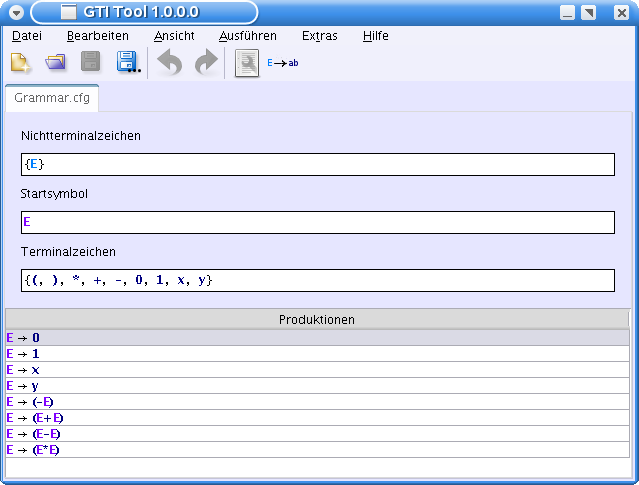
\includegraphics[width=12cm]{../images/cfg_example.png}
\caption{Grammatik}
\label{FigureProduction}
\end{center}
\end{figure}
\vspace{10pt}

Zur Darstellung der Produktionen wird eine Listenansicht verwendet, wobei die
Produktionen als Pretty-String angezeigt werden, welche ja schon in Abschnitt
\ref{GUIDesign} beschrieben wurden. Wir hoffen, dadurch eine bessere
Übersichtlichkeit in den einzelnen Produktionen für den Benutzer geschaffen zu haben (siehe Abbildung
\ref{FigureProduction}).\vspace{10pt}

Als Hilfestellung beim Anlegen von neuen Produktionen wird die aktuelle
Konfiguration der Grammatik oberhalb der existierenden Produktionen
angezeigt.\vspace{10pt}


\begin{figure}[h!]
\begin{center}
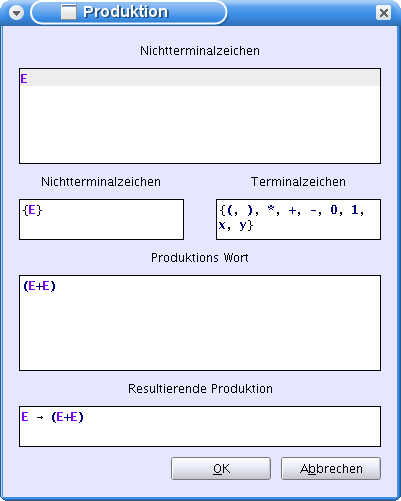
\includegraphics[width=8cm]{../images/production_dialog.png}
\caption{Produktion anlegen}
\label{FigureAddProduction}
\end{center}
\end{figure}
\vspace{10pt}

Wir haben versucht, das Anlegen einer neuen Produktion so intuitiv wie möglich
zu gestalten. Der Benutzer kann das Nichtterminalzeichen, welches die linke
Seite der Produktion repräsentiert, anhand einer Liste der
verfügbaren Symbole auswählen. Die Eingabe der rechten Seite ist
wieder über ein Textfeld, mit entsprechendem Parser, realisiert
worden. Oberhalb des Eingabefeldes wird dabei angezeigt, welche Symbole zur
Konstruktion des Wortes der Satzform zur Verfügung stehen. Als weitere
Hilfestellung haben wir unterhalb des Eingabefeldes einen Bereich angelegt,
in welchem die resultierende Produktion angezeigt wird. So kann der
Benuzter jederzeit überprüfen, ob das Ergebnis seinen
Vorstellungen entspricht. In Abbildung \ref{FigureAddProduction}
sieht man den Dialog, welcher verwendet wird, um Produktionen
anzulegen und zu bearbeiten.\vspace{10pt}

Der Benutzer hat auch die Möglichkeit, seine definierte Grammatik zu validieren.
Abschnitt \ref{InteractionGrammar} beschreibt die Umsetzung im
Detail.\vspace{10pt}


\section{Konvertierung}\label{ConverToGrammar}

Wenn ein Benutzer eine Grammatik vollständig erstellt hat, kann es durchaus
interessant sein, den Automaten zu sehen, welcher die Sprache akzeptiert, die
durch die Grammatik beschrieben wird. Vor allem, da für Automaten weitaus mehr
Verwendungsmöglichkeiten in diesem Werkzeug existieren.\vspace{10pt}


\subsection{Konvertierung einer regulären Grammatik}\label{ConverToGrammarRegular}

Eine reguläre Grammatik kann in einen entsprechenden nichtdeterministischen,
endlichen Automaten umgewandelt werden. Der verwendete Algorithmus kann in
\cite{Compilers} nachgelesen werden. Die Zustände unseres entstehenden Automaten
resultieren aus den Nichtterminalzeichen unserer Grammatik. Allerdings werden in
der Implementierung nur Zustände für die Nichtterminalzeichen angelegt, welche
auch in einer Produktion, auf der rechten oder linken Seite, verwendet werden.
Die Zustände werden immer dann angelegt, wenn man auf ein Nichtterminalzeichen
trifft, welches man bis jetzt noch nicht gesehen hat.\vspace{10pt}

Die rechte Seite einer Produktion kann entweder aus einem einzelnen
Terminalzeichen (z.B. $\NonterminalSymbol{S} \to \TerminalSymbol{a}$), oder
aus einem Terminalzeichen mit einem anschließenden Nichtterminalzeichen
(z.B. $\NonterminalSymbol{S} \to \TerminalSymbol{a}\NonterminalSymbol{A}$)
bestehen, da nur solche Arten von Produktionen in einer rechtsregulären
Grammatik zugelassen sind.\vspace{10pt}

Am Anfang legen wir einen akzeptierenden Zustand an, welchen wir im weitern
Verlauf des Algorithmus noch benötigen werden.\vspace{10pt}

Wir betrachten jede Produktion der Grammatik. Zunächst interessiert uns die linke
Seite. Wenn wir das Nichtterminalzeichen bereits gesehen haben, wurde auch schon
ein Zustand dafür angelegt, und wir merken uns diesen. Wenn wir das
Nichtterminalzeichen noch nicht gesehen haben, müssen wir jetzt einen neuen
Zustand anlegen, welcher dieses repräsentiert, und merken uns diesen neuen
Zustand, da dieser der Ausgangszustand für die zu erstellenden Übergänge
ist.\vspace{10pt}

Als nächstes betrachten wir die rechte Seite der Produktion. Wenn es sich dabei
um ein einzelnes Terminalzeichen handelt, wird ein Übergang von dem Zustand für
das Nichtterminalzeichen zu dem akzeptierenden Zustand erzeugt, wobei die
Übergangsmenge aus dem Terminalzeichen auf der rechten Seite der Produktion
besteht.\vspace{10pt}

Besteht die rechte Seite allerdings aus einem Terminalzeichen und einem
Nichtterminalzeichen müssen wir wieder überprüfen, ob wir das
Nichtterminalzeichen bereits gesehen haben, um gegebenenfalls den
entsprechenden Zustand anzulegen. Im nächsten Schritt wird ein Übergang,
zwischen den beiden Zuständen die wir uns gemerkt haben, angelegt, mit der
rechten Seite der Produktion als Übergangsmenge.\vspace{10pt}

Diese Behandlung wiederholen wir für jede Produktion der Grammatik und
erhalten so einen endlichen Automaten, der genau die von der
Grammatik erzeugte Sprache akzeptiert.\vspace{10pt}


\subsection{Konvertierung einer kontextfreien Grammatik}\label{ConverToGrammarContextFree}

Der Benutzer hat auch die Möglichkeit, eine zuvor erstellte kontextfreie
Grammatik in einen Kellerautomaten umwandeln zu lassen. Dieser
Algorithmus ist in \cite{Compilers} beschrieben\vspace{10pt}

Zu Beginn werden zwei Zustände angelegt, ein Startzustand und ein
akzeptierender Zustand. Dazu wird ein Übergang vom Startzustand in den
akzeptierenden Zustand angelegt, welcher das Startsymbol der Grammatik in den
Keller legt. Dann wird für jede Produktion ein Übergang angelegt, welcher die rechte
Seite der Produktion vom Keller entfernt, und dafür die linke Seite der
Produktion auf den Keller schreibt. Dieser Übergang hat als
Ursprungs- und Zielzustand den akzeptierenden Zustand.\vspace{10pt}

Wenn alle Produktionen verarbeitet wurden, wird zusätzlich pro Terminalzeichen
ein Übergang vom akzeptierenden Zustand in sich selbst angelegt.
In jedem dieser Übergänge wird das entsprechende Terminalzeichen vom Eingabeband
gelesen und vom Keller des Automaten genommen.\vspace{10pt}

Durch die Zweite Ansicht (siehe Abschnitt \ref{SecondView}) hat der Benuzter
auch die Möglichkeit, die Ausgangsgrammatik und den enstandenen Automaten
nebeneinander zu sehen, um die Zusammenhänge besser verstehen zu können.\vspace{10pt}


\section{Fehler und Warnungen}\label{InteractionGrammar}

Im Folgenden möchten wir auf die Fehler und Warnungen eingehen, welche bei dem
Validierungsvorgang einer Grammatik auftreten können.\vspace{10pt}

Zu diesen Validierungsfehlern zählt unter anderem, wenn die selbe Produktion
mehrfach in einer Grammatik existiert. In der Spalte "`Meldung"' sieht man wie
immer nur, um welchen Fehler es sich gerade handelt. Über die Beschreibung wird
mitgeteilt, um welche Produktion es sich dabei handelt.\vspace{10pt}

Handelt es sich bei der aktuellen Grammatik um eine reguläre Grammatik, gibt es
noch eine weitere Fehlermeldung. Wenn nicht alle Produktionen den vorgegebenen
Satzformen für eine rechtsreguläre Grammtik entsprechen, wird dies auch durch
einen Validierungsfehler angezeigt. Dabei kann man auch hier anhand der
Beschreibung sehen, um welche Produktion es sich handelt. Wenn man den
entsprechenden Eintrag auswählt, wird dem Benutzer wieder durch farbiges
Hervorheben signalisiert, wo sich diese Produktion befindet. Es wird jetzt
allerdings nicht die ganze Produktion eingefärbt, sondern nur der Teil der
Satzform, welcher nicht den Satzformen für reguläre Grammatiken entspricht.\vspace{10pt}

Neben diesen beiden Fehlern haben wir auch eine Warnung eingeführt. Diese gibt
Auskunft darüber, wenn ein Nichtterminalzeichen, vom Startsymbol ausgehend, nicht
Teil einer ableitbaren Satzform ist. Es handelt sich hierbei nur um eine Warnung,
weil es sich durchaus um eine gültige Grammatik handeln kann. Sie soll dem
Benutzer allerdings dazu animieren, die Produktionsmenge zu kontrollieren, ob
nicht eine oder mehrere Produktionen vergessen wurden. So soll es möglich sein,
Flüchtig\-keits\-fehler frühzeitig zu erkennen und zu beheben.\vspace{10pt}


%### removes texlipse warnings
